%%%%%%%%%%%%%%%%%%%%%%%%%%%%%%%%%%%%%%%%%
% Masters/Doctoral Thesis 
% LaTeX Template
% Version 2.5 (27/8/17)
%
% This template was downloaded from:
% http://www.LaTeXTemplates.com
%
% Version 2.x major modifications by:
% Vel (vel@latextemplates.com)
%
% This template is based on a template by:
% Steve Gunn (http://users.ecs.soton.ac.uk/srg/softwaretools/document/templates/)
% Sunil Patel (http://www.sunilpatel.co.uk/thesis-template/)
%
% Template license:
% CC BY-NC-SA 3.0 (http://creativecommons.org/licenses/by-nc-sa/3.0/)
%
%%%%%%%%%%%%%%%%%%%%%%%%%%%%%%%%%%%%%%%%%

%----------------------------------------------------------------------------------------
%	PACKAGES AND OTHER DOCUMENT CONFIGURATIONS
%----------------------------------------------------------------------------------------

\documentclass[
11pt, % The default document font size, options: 10pt, 11pt, 12pt
%oneside, % Two side (alternating margins) for binding by default, uncomment to switch to one side
spanish, % ngerman for German
singlespacing, % Single line spacing, alternatives: onehalfspacing or doublespacing
%draft, % Uncomment to enable draft mode (no pictures, no links, overfull hboxes indicated)
%nolistspacing, % If the document is onehalfspacing or doublespacing, uncomment this to set spacing in lists to single
%liststotoc, % Uncomment to add the list of figures/tables/etc to the table of contents
%toctotoc, % Uncomment to add the main table of contents to the table of contents
%parskip, % Uncomment to add space between paragraphs
%nohyperref, % Uncomment to not load the hyperref package
headsepline, % Uncomment to get a line under the header
%chapterinoneline, % Uncomment to place the chapter title next to the number on one line
%consistentlayout, % Uncomment to change the layout of the declaration, abstract and acknowledgements pages to match the default layout
]{MastersDoctoralThesis} % The class file specifying the document structure

\usepackage[utf8]{inputenc} % Required for inputting international characters
\usepackage[T1]{fontenc} % Output font encoding for international characters

\usepackage{mathpazo} % Use the Palatino font by default
\usepackage{tikz}
\usetikzlibrary{shapes,arrows}
\usetikzlibrary{babel}
\usetikzlibrary{positioning,fit,calc}
\usepackage{multirow}
\usepackage{textcomp}

\usepackage[backend=biber,style=authoryear,natbib=true]{biblatex} % Use the bibtex backend with the authoryear citation style (which resembles APA)

\addbibresource{bib.bib} % The filename of the bibliography

\usepackage[autostyle=true]{csquotes} % Required to generate language-dependent quotes in the bibliography

%----------------------------------------------------------------------------------------
%	MARGIN SETTINGS
%----------------------------------------------------------------------------------------

\geometry{
	paper=letterpaper, % Change to letterpaper for US letter
	inner=2.5cm, % Inner margin
	outer=3.8cm, % Outer margin
	bindingoffset=.5cm, % Binding offset
	top=1.5cm, % Top margin
	bottom=1.5cm, % Bottom margin
	%showframe, % Uncomment to show how the type block is set on the page
}

%----------------------------------------------------------------------------------------
%	THESIS INFORMATION
%----------------------------------------------------------------------------------------

\thesistitle{Silla de ruedas motorizada} % Your thesis title, this is used in the title and abstract, print it elsewhere with \ttitle
\supervisor{Dr. Adri\'an \textsc{Espinoza}} % Your supervisor's name, this is used in the title page, print it elsewhere with \supname
\examiner{} % Your examiner's name, this is not currently used anywhere in the template, print it elsewhere with \examname
\degree{Seminario de Ingenier\'ia} % Your degree name, this is used in the title page and abstract, print it elsewhere with \degreename
\author{Jes\'us \textsc{Montes}\\ Angel \textsc{Ram\'irez}} % Your name, this is used in the title page and abstract, print it elsewhere with \authorname
\addresses{} % Your address, this is not currently used anywhere in the template, print it elsewhere with \addressname

\subject{Mecatr\'onica} % Your subject area, this is not currently used anywhere in the template, print it elsewhere with \subjectname
\keywords{} % Keywords for your thesis, this is not currently used anywhere in the template, print it elsewhere with \keywordnames
\university{\href{https://www.unam.mx}{Universidad Nacional Aut\'onoma de
M\'exico}} % Your university's name and URL, this is used in the title page and abstract, print it elsewhere with \univname
\department{\href{http://www.ingenieria.unam.mx/dimei}{Divisi\'on de Ingenier\'ia
Mec\'anica e Industrial}} % Your department's name and URL, this is used in the title page and abstract, print it elsewhere with \deptname
\group{\href{http://www.ingenieria.unam.mx/dimei/proyecto_seminario_ingenieria.php}{Seminario de Ingenier\'ia}} % Your research group's name and URL, this is used in the title page, print it elsewhere with \groupname
\faculty{\href{http://www.ingenieria.unam.mx}{Facultad de Ingenier\'ia}} % Your faculty's name and URL, this is used in the title page and abstract, print it elsewhere with \facname

\AtBeginDocument{
\hypersetup{pdftitle=\ttitle} % Set the PDF's title to your title
\hypersetup{pdfauthor=\authorname} % Set the PDF's author to your name
\hypersetup{pdfkeywords=\keywordnames} % Set the PDF's keywords to your keywords
}

\begin{document}

\frontmatter % Use roman page numbering style (i, ii, iii, iv...) for the pre-content pages

\pagestyle{plain} % Default to the plain heading style until the thesis style is called for the body content

%----------------------------------------------------------------------------------------
%	TITLE PAGE
%----------------------------------------------------------------------------------------

\begin{titlepage}
\begin{center}

\vspace*{.06\textheight}
{\scshape\LARGE \univname\par}\vspace{1.5cm} % University name
\textsc{\Large Facultad de Ingenier\'ia}\\[0.5cm] % Thesis type

\HRule \\[0.4cm] % Horizontal line
{\huge \bfseries \ttitle\par}\vspace{0.4cm} % Thesis title
\HRule \\[1.5cm] % Horizontal line
 
\begin{minipage}[t]{0.4\textwidth}
\begin{flushleft} \large
\emph{Autor:}\\
{\authorname} % Author name - remove the \href bracket to remove the link
\end{flushleft}
\end{minipage}
\begin{minipage}[t]{0.4\textwidth}
\begin{flushright} \large
\emph{Supervisor:} \\
{\supname} % Supervisor name - remove the \href bracket to remove the link  
\end{flushright}
\end{minipage}\\[3cm]
 
\vfill

\large \textit{Qu\'e con la finalidad de acreditar la materia}\\[0.3cm] % University requirement text
\textit{de}\\[0.4cm]
\groupname\\\deptname\\[2cm] % Research group name and department name
 
\vfill

{\large \today}\\[4cm] % Date
%\includegraphics{Logo} % University/department logo - uncomment to place it
 
\vfill
\end{center}
\end{titlepage}

%----------------------------------------------------------------------------------------
%	DECLARATION PAGE
%----------------------------------------------------------------------------------------

% \begin{declaration}
% \addchaptertocentry{\authorshipname} % Add the declaration to the table of contents
% \noindent I, \authorname, declare that this thesis titled, \enquote{\ttitle} and the work presented in it are my own. I confirm that:

% \begin{itemize} 
% \item This work was done wholly or mainly while in candidature for a research degree at this University.
% \item Where any part of this thesis has previously been submitted for a degree or any other qualification at this University or any other institution, this has been clearly stated.
% \item Where I have consulted the published work of others, this is always clearly attributed.
% \item Where I have quoted from the work of others, the source is always given. With the exception of such quotations, this thesis is entirely my own work.
% \item I have acknowledged all main sources of help.
% \item Where the thesis is based on work done by myself jointly with others, I have made clear exactly what was done by others and what I have contributed myself.\\
% \end{itemize}
 
% \noindent Signed:\\
% \rule[0.5em]{25em}{0.5pt} % This prints a line for the signature
 
% \noindent Date:\\
% \rule[0.5em]{25em}{0.5pt} % This prints a line to write the date
% \end{declaration}

\cleardoublepage

%----------------------------------------------------------------------------------------
%	QUOTATION PAGE
%----------------------------------------------------------------------------------------

% \vspace*{0.2\textheight}

% \noindent\enquote{\itshape Thanks to my solid academic training, today I can write hundreds of words on virtually any topic without possessing a shred of information, which is how I got a good job in journalism.}\bigbreak

% \hfill Dave Barry

%----------------------------------------------------------------------------------------
%	ABSTRACT PAGE
%----------------------------------------------------------------------------------------

\begin{abstract}
\addchaptertocentry{\abstractname} % Add the abstract to the table of contents
The Thesis Abstract is written here (and usually kept to just this page). The page is kept centered vertically so can expand into the blank space above the title too\ldots
\end{abstract}

%----------------------------------------------------------------------------------------
%	ACKNOWLEDGEMENTS
%----------------------------------------------------------------------------------------

% \begin{acknowledgements}
% \addchaptertocentry{\acknowledgementname} % Add the acknowledgements to the table of contents
% The acknowledgments and the people to thank go here, don't forget to include your project advisor\ldots
% \end{acknowledgements}

%----------------------------------------------------------------------------------------
%	LIST OF CONTENTS/FIGURES/TABLES PAGES
%----------------------------------------------------------------------------------------

\tableofcontents % Prints the main table of contents

\listoffigures % Prints the list of figures

\listoftables % Prints the list of tables

%----------------------------------------------------------------------------------------
%	ABBREVIATIONS
%----------------------------------------------------------------------------------------

% \begin{abbreviations}{ll} % Include a list of abbreviations (a table of two columns)

% \textbf{LAH} & \textbf{L}ist \textbf{A}bbreviations \textbf{H}ere\\
% \textbf{WSF} & \textbf{W}hat (it) \textbf{S}tands \textbf{F}or\\

% \end{abbreviations}

%----------------------------------------------------------------------------------------
%	PHYSICAL CONSTANTS/OTHER DEFINITIONS
%----------------------------------------------------------------------------------------

%\begin{constants}{lr@{${}={}$}l} % The list of physical constants is a three column table

%% The \SI{}{} command is provided by the siunitx package, see its documentation for instructions on how to use it

%Speed of Light & $c_{0}$ & \SI{2.99792458e8}{\meter\per\second} (exact)\\
%%Constant Name & $Symbol$ & $Constant Value$ with units\\

%\end{constants}

%%----------------------------------------------------------------------------------------
%%	SYMBOLS
%%----------------------------------------------------------------------------------------

%\begin{symbols}{lll} % Include a list of Symbols (a three column table)

%$a$ & distance & \si{\meter} \\
%$P$ & power & \si{\watt} (\si{\joule\per\second}) \\
%%Symbol & Name & Unit \\

%\addlinespace % Gap to separate the Roman symbols from the Greek

%$\omega$ & angular frequency & \si{\radian} \\

%\end{symbols}

%----------------------------------------------------------------------------------------
%	DEDICATION
%----------------------------------------------------------------------------------------

% \dedicatory{Un espacial agradecimiento a\ldots} 

%----------------------------------------------------------------------------------------
%	THESIS CONTENT - CHAPTERS
%----------------------------------------------------------------------------------------

\mainmatter % Begin numeric (1,2,3...) page numbering

\pagestyle{thesis} % Return the page headers back to the "thesis" style

% Include the chapters of the thesis as separate files from the Chapters folder
% Uncomment the lines as you write the chapters

% Chapter 1

\chapter{Introducci\'on} % Main chapter title

\label{Chapter1} % For referencing the chapter elsewhere, use \ref{Chapter1} 

%----------------------------------------------------------------------------------------

% Define some commands to keep the formatting separated from the content 
\newcommand{\keyword}[1]{\textbf{#1}}
\newcommand{\tabhead}[1]{\textbf{#1}}
\newcommand{\code}[1]{\texttt{#1}}
\newcommand{\file}[1]{\texttt{\bfseries#1}}
\newcommand{\option}[1]{\texttt{\itshape#1}}

%----------------------------------------------------------------------------------------

\section{Estado del arte}
Welcome to this \LaTeX{} Thesis Template, a beautiful and easy to use template for writing a thesis using the \LaTeX{} typesetting system.

If you are writing a thesis (or will be in the future) and its subject is technical or mathematical (though it doesn't have to be), then creating it in \LaTeX{} is highly recommended as a way to make sure you can just get down to the essential writing without having to worry over formatting or wasting time arguing with your word processor. 

\LaTeX{} is easily able to professionally typeset documents that run to hundreds or thousands of pages long. With simple mark-up commands, it automatically sets out the table of contents, margins, page headers and footers and keeps the formatting consistent and beautiful. One of its main strengths is the way it can easily typeset mathematics, even \emph{heavy} mathematics. Even if those equations are the most horribly twisted and most difficult mathematical problems that can only be solved on a super-computer, you can at least count on \LaTeX{} to make them look stunning.

%----------------------------------------------------------------------------------------

\section{Breve historia de las sillas de ruedas}

\LaTeX{} is not a \textsc{wysiwyg} (What You See is What You Get) program, unlike word processors such as Microsoft Word or Apple's Pages. Instead, a document written for \LaTeX{} is actually a simple, plain text file that contains \emph{no formatting}. You tell \LaTeX{} how you want the formatting in the finished document by writing in simple commands amongst the text, for example, if I want to use \emph{italic text for emphasis}, I write the \verb|\emph{text}| command and put the text I want in italics in between the curly braces. This means that \LaTeX{} is a \enquote{mark-up} language, very much like HTML.

\subsection{A (not so short) Introduction to \LaTeX{}}

If you are new to \LaTeX{}, there is a very good eBook -- freely available online as a PDF file -- called, \enquote{The Not So Short Introduction to \LaTeX{}}. The book's title is typically shortened to just \emph{lshort}. You can download the latest version (as it is occasionally updated) from here:
\url{http://www.ctan.org/tex-archive/info/lshort/english/lshort.pdf}

It is also available in several other languages. Find yours from the list on this page: \url{http://www.ctan.org/tex-archive/info/lshort/}

It is recommended to take a little time out to learn how to use \LaTeX{} by creating several, small `test' documents, or having a close look at several templates on:\\ 
\url{http://www.LaTeXTemplates.com}\\ 
Making the effort now means you're not stuck learning the system when what you \emph{really} need to be doing is writing your thesis.

\subsection{A Short Math Guide for \LaTeX{}}

If you are writing a technical or mathematical thesis, then you may want to read the document by the AMS (American Mathematical Society) called, \enquote{A Short Math Guide for \LaTeX{}}. It can be found online here:
\url{http://www.ams.org/tex/amslatex.html}
under the \enquote{Additional Documentation} section towards the bottom of the page.

\subsection{Common \LaTeX{} Math Symbols}
There are a multitude of mathematical symbols available for \LaTeX{} and it would take a great effort to learn the commands for them all. The most common ones you are likely to use are shown on this page:
\url{http://www.sunilpatel.co.uk/latex-type/latex-math-symbols/}

You can use this page as a reference or crib sheet, the symbols are rendered as large, high quality images so you can quickly find the \LaTeX{} command for the symbol you need.

\subsection{\LaTeX{} on a Mac}
 
The \LaTeX{} distribution is available for many systems including Windows, Linux and Mac OS X. The package for OS X is called MacTeX and it contains all the applications you need -- bundled together and pre-customized -- for a fully working \LaTeX{} environment and work flow.
 
MacTeX includes a custom dedicated \LaTeX{} editor called TeXShop for writing your `\file{.tex}' files and BibDesk: a program to manage your references and create your bibliography section just as easily as managing songs and creating playlists in iTunes.

%----------------------------------------------------------------------------------------

\section{Implicaciones m\'edicas}

If you are familiar with \LaTeX{}, then you should explore the directory structure of the template and then proceed to place your own information into the \emph{THESIS INFORMATION} block of the \file{main.tex} file. You can then modify the rest of this file to your unique specifications based on your degree/university. Section \ref{FillingFile} on page \pageref{FillingFile} will help you do this. Make sure you also read section \ref{ThesisConventions} about thesis conventions to get the most out of this template.

If you are new to \LaTeX{} it is recommended that you carry on reading through the rest of the information in this document.

Before you begin using this template you should ensure that its style complies with the thesis style guidelines imposed by your institution. In most cases this template style and layout will be suitable. If it is not, it may only require a small change to bring the template in line with your institution's recommendations. These modifications will need to be done on the \file{MastersDoctoralThesis.cls} file.

\subsection{About this Template}

This \LaTeX{} Thesis Template is originally based and created around a \LaTeX{} style file created by Steve R.\ Gunn from the University of Southampton (UK), department of Electronics and Computer Science. You can find his original thesis style file at his site, here:
\url{http://www.ecs.soton.ac.uk/~srg/softwaretools/document/templates/}

Steve's \file{ecsthesis.cls} was then taken by Sunil Patel who modified it by creating a skeleton framework and folder structure to place the thesis files in. The resulting template can be found on Sunil's site here:
\url{http://www.sunilpatel.co.uk/thesis-template}

Sunil's template was made available through \url{http://www.LaTeXTemplates.com} where it was modified many times based on user requests and questions. Version 2.0 and onwards of this template represents a major modification to Sunil's template and is, in fact, hardly recognisable. The work to make version 2.0 possible was carried out by \href{mailto:vel@latextemplates.com}{Vel} and Johannes Böttcher.

%----------------------------------------------------------------------------------------

\section{Sensores y actuadores}

\subsection{Folders}

This template comes as a single zip file that expands out to several files and folders. The folder names are mostly self-explanatory:

\keyword{Appendices} -- this is the folder where you put the appendices. Each appendix should go into its own separate \file{.tex} file. An example and template are included in the directory.

\keyword{Chapters} -- this is the folder where you put the thesis chapters. A thesis usually has about six chapters, though there is no hard rule on this. Each chapter should go in its own separate \file{.tex} file and they can be split as:
\begin{itemize}
\item Chapter 1: Introduction to the thesis topic
\item Chapter 2: Background information and theory
\item Chapter 3: (Laboratory) experimental setup
\item Chapter 4: Details of experiment 1
\item Chapter 5: Details of experiment 2
\item Chapter 6: Discussion of the experimental results
\item Chapter 7: Conclusion and future directions
\end{itemize}
This chapter layout is specialised for the experimental sciences, your discipline may be different.

\keyword{Figures} -- this folder contains all figures for the thesis. These are the final images that will go into the thesis document.

\subsection{Files}

Included are also several files, most of them are plain text and you can see their contents in a text editor. After initial compilation, you will see that more auxiliary files are created by \LaTeX{} or BibTeX and which you don't need to delete or worry about:

\keyword{example.bib} -- this is an important file that contains all the bibliographic information and references that you will be citing in the thesis for use with BibTeX. You can write it manually, but there are reference manager programs available that will create and manage it for you. Bibliographies in \LaTeX{} are a large subject and you may need to read about BibTeX before starting with this. Many modern reference managers will allow you to export your references in BibTeX format which greatly eases the amount of work you have to do.

\keyword{MastersDoctoralThesis.cls} -- this is an important file. It is the class file that tells \LaTeX{} how to format the thesis. 

\keyword{main.pdf} -- this is your beautifully typeset thesis (in the PDF file format) created by \LaTeX{}. It is supplied in the PDF with the template and after you compile the template you should get an identical version.

\keyword{main.tex} -- this is an important file. This is the file that you tell \LaTeX{} to compile to produce your thesis as a PDF file. It contains the framework and constructs that tell \LaTeX{} how to layout the thesis. It is heavily commented so you can read exactly what each line of code does and why it is there. After you put your own information into the \emph{THESIS INFORMATION} block -- you have now started your thesis!

Files that are \emph{not} included, but are created by \LaTeX{} as auxiliary files include:

\keyword{main.aux} -- this is an auxiliary file generated by \LaTeX{}, if it is deleted \LaTeX{} simply regenerates it when you run the main \file{.tex} file.

\keyword{main.bbl} -- this is an auxiliary file generated by BibTeX, if it is deleted, BibTeX simply regenerates it when you run the \file{main.aux} file. Whereas the \file{.bib} file contains all the references you have, this \file{.bbl} file contains the references you have actually cited in the thesis and is used to build the bibliography section of the thesis.

\keyword{main.blg} -- this is an auxiliary file generated by BibTeX, if it is deleted BibTeX simply regenerates it when you run the main \file{.aux} file.

\keyword{main.lof} -- this is an auxiliary file generated by \LaTeX{}, if it is deleted \LaTeX{} simply regenerates it when you run the main \file{.tex} file. It tells \LaTeX{} how to build the \emph{List of Figures} section.

\keyword{main.log} -- this is an auxiliary file generated by \LaTeX{}, if it is deleted \LaTeX{} simply regenerates it when you run the main \file{.tex} file. It contains messages from \LaTeX{}, if you receive errors and warnings from \LaTeX{}, they will be in this \file{.log} file.

\keyword{main.lot} -- this is an auxiliary file generated by \LaTeX{}, if it is deleted \LaTeX{} simply regenerates it when you run the main \file{.tex} file. It tells \LaTeX{} how to build the \emph{List of Tables} section.

\keyword{main.out} -- this is an auxiliary file generated by \LaTeX{}, if it is deleted \LaTeX{} simply regenerates it when you run the main \file{.tex} file.

So from this long list, only the files with the \file{.bib}, \file{.cls} and \file{.tex} extensions are the most important ones. The other auxiliary files can be ignored or deleted as \LaTeX{} and BibTeX will regenerate them.

%----------------------------------------------------------------------------------------

\section{Sistemas de energ\'ia}\label{FillingFile}

You will need to personalise the thesis template and make it your own by filling in your own information. This is done by editing the \file{main.tex} file in a text editor or your favourite LaTeX environment.

Open the file and scroll down to the third large block titled \emph{THESIS INFORMATION} where you can see the entries for \emph{University Name}, \emph{Department Name}, etc \ldots

Fill out the information about yourself, your group and institution. You can also insert web links, if you do, make sure you use the full URL, including the \code{http://} for this. If you don't want these to be linked, simply remove the \verb|\href{url}{name}| and only leave the name.

When you have done this, save the file and recompile \code{main.tex}. All the information you filled in should now be in the PDF, complete with web links. You can now begin your thesis proper!

%----------------------------------------------------------------------------------------

\section{Interfaces}

The \file{main.tex} file contains the structure of the thesis. There are plenty of written comments that explain what pages, sections and formatting the \LaTeX{} code is creating. Each major document element is divided into commented blocks with titles in all capitals to make it obvious what the following bit of code is doing. Initially there seems to be a lot of \LaTeX{} code, but this is all formatting, and it has all been taken care of so you don't have to do it.

Begin by checking that your information on the title page is correct. For the thesis declaration, your institution may insist on something different than the text given. If this is the case, just replace what you see with what is required in the \emph{DECLARATION PAGE} block.

Then comes a page which contains a funny quote. You can put your own, or quote your favourite scientist, author, person, and so on. Make sure to put the name of the person who you took the quote from.

Following this is the abstract page which summarises your work in a condensed way and can almost be used as a standalone document to describe what you have done. The text you write will cause the heading to move up so don't worry about running out of space.

Next come the acknowledgements. On this page, write about all the people who you wish to thank (not forgetting parents, partners and your advisor/supervisor).

The contents pages, list of figures and tables are all taken care of for you and do not need to be manually created or edited. The next set of pages are more likely to be optional and can be deleted since they are for a more technical thesis: insert a list of abbreviations you have used in the thesis, then a list of the physical constants and numbers you refer to and finally, a list of mathematical symbols used in any formulae. Making the effort to fill these tables means the reader has a one-stop place to refer to instead of searching the internet and references to try and find out what you meant by certain abbreviations or symbols.

The list of symbols is split into the Roman and Greek alphabets. Whereas the abbreviations and symbols ought to be listed in alphabetical order (and this is \emph{not} done automatically for you) the list of physical constants should be grouped into similar themes.

The next page contains a one line dedication. Who will you dedicate your thesis to?

Finally, there is the block where the chapters are included. Uncomment the lines (delete the \code{\%} character) as you write the chapters. Each chapter should be written in its own file and put into the \emph{Chapters} folder and named \file{Chapter1}, \file{Chapter2}, etc\ldots Similarly for the appendices, uncomment the lines as you need them. Each appendix should go into its own file and placed in the \emph{Appendices} folder.

After the preamble, chapters and appendices finally comes the bibliography. The bibliography style (called \option{authoryear}) is used for the bibliography and is a fully featured style that will even include links to where the referenced paper can be found online. Do not underestimate how grateful your reader will be to find that a reference to a paper is just a click away. Of course, this relies on you putting the URL information into the BibTeX file in the first place.

%----------------------------------------------------------------------------------------

\section{Thesis Features and Conventions}\label{ThesisConventions}

To get the best out of this template, there are a few conventions that you may want to follow.

One of the most important (and most difficult) things to keep track of in such a long document as a thesis is consistency. Using certain conventions and ways of doing things (such as using a Todo list) makes the job easier. Of course, all of these are optional and you can adopt your own method.

\subsection{Printing Format}

This thesis template is designed for double sided printing (i.e. content on the front and back of pages) as most theses are printed and bound this way. Switching to one sided printing is as simple as uncommenting the \option{oneside} option of the \code{documentclass} command at the top of the \file{main.tex} file. You may then wish to adjust the margins to suit specifications from your institution.

The headers for the pages contain the page number on the outer side (so it is easy to flick through to the page you want) and the chapter name on the inner side.

The text is set to 11 point by default with single line spacing, again, you can tune the text size and spacing should you want or need to using the options at the very start of \file{main.tex}. The spacing can be changed similarly by replacing the \option{singlespacing} with \option{onehalfspacing} or \option{doublespacing}.

\subsection{Using US Letter Paper}

The paper size used in the template is A4, which is the standard size in Europe. If you are using this thesis template elsewhere and particularly in the United States, then you may have to change the A4 paper size to the US Letter size. This can be done in the margins settings section in \file{main.tex}.

Due to the differences in the paper size, the resulting margins may be different to what you like or require (as it is common for institutions to dictate certain margin sizes). If this is the case, then the margin sizes can be tweaked by modifying the values in the same block as where you set the paper size. Now your document should be set up for US Letter paper size with suitable margins.

\subsection{References}

The \code{biblatex} package is used to format the bibliography and inserts references such as this one \parencite{Reference1}. The options used in the \file{main.tex} file mean that the in-text citations of references are formatted with the author(s) listed with the date of the publication. Multiple references are separated by semicolons (e.g. \parencite{Reference2, Reference1}) and references with more than three authors only show the first author with \emph{et al.} indicating there are more authors (e.g. \parencite{Reference3}). This is done automatically for you. To see how you use references, have a look at the \file{Chapter1.tex} source file. Many reference managers allow you to simply drag the reference into the document as you type.

Scientific references should come \emph{before} the punctuation mark if there is one (such as a comma or period). The same goes for footnotes\footnote{Such as this footnote, here down at the bottom of the page.}. You can change this but the most important thing is to keep the convention consistent throughout the thesis. Footnotes themselves should be full, descriptive sentences (beginning with a capital letter and ending with a full stop). The APA6 states: \enquote{Footnote numbers should be superscripted, [...], following any punctuation mark except a dash.} The Chicago manual of style states: \enquote{A note number should be placed at the end of a sentence or clause. The number follows any punctuation mark except the dash, which it precedes. It follows a closing parenthesis.}

The bibliography is typeset with references listed in alphabetical order by the first author's last name. This is similar to the APA referencing style. To see how \LaTeX{} typesets the bibliography, have a look at the very end of this document (or just click on the reference number links in in-text citations).

\subsubsection{A Note on bibtex}

The bibtex backend used in the template by default does not correctly handle unicode character encoding (i.e. "international" characters). You may see a warning about this in the compilation log and, if your references contain unicode characters, they may not show up correctly or at all. The solution to this is to use the biber backend instead of the outdated bibtex backend. This is done by finding this in \file{main.tex}: \option{backend=bibtex} and changing it to \option{backend=biber}. You will then need to delete all auxiliary BibTeX files and navigate to the template directory in your terminal (command prompt). Once there, simply type \code{biber main} and biber will compile your bibliography. You can then compile \file{main.tex} as normal and your bibliography will be updated. An alternative is to set up your LaTeX editor to compile with biber instead of bibtex, see \href{http://tex.stackexchange.com/questions/154751/biblatex-with-biber-configuring-my-editor-to-avoid-undefined-citations/}{here} for how to do this for various editors.

\subsection{Tables}

Tables are an important way of displaying your results, below is an example table which was generated with this code:

{\small
\begin{verbatim}
\begin{table}
\caption{The effects of treatments X and Y on the four groups studied.}
\label{tab:treatments}
\centering
\begin{tabular}{l l l}
\toprule
\tabhead{Groups} & \tabhead{Treatment X} & \tabhead{Treatment Y} \\
\midrule
1 & 0.2 & 0.8\\
2 & 0.17 & 0.7\\
3 & 0.24 & 0.75\\
4 & 0.68 & 0.3\\
\bottomrule\\
\end{tabular}
\end{table}
\end{verbatim}
}

\begin{table}
\caption{The effects of treatments X and Y on the four groups studied.}
\label{tab:treatments}
\centering
\begin{tabular}{l l l}
\toprule
\tabhead{Groups} & \tabhead{Treatment X} & \tabhead{Treatment Y} \\
\midrule
1 & 0.2 & 0.8\\
2 & 0.17 & 0.7\\
3 & 0.24 & 0.75\\
4 & 0.68 & 0.3\\
\bottomrule\\
\end{tabular}
\end{table}

You can reference tables with \verb|\ref{<label>}| where the label is defined within the table environment. See \file{Chapter1.tex} for an example of the label and citation (e.g. Table~\ref{tab:treatments}).

\subsection{Figures}

There will hopefully be many figures in your thesis (that should be placed in the \emph{Figures} folder). The way to insert figures into your thesis is to use a code template like this:
\begin{verbatim}
\begin{figure}
\centering

\includegraphics{Figures/Electron}
\decoRule
\caption[An Electron]{An electron (artist's impression).}
\label{fig:Electron}
\end{figure}
\end{verbatim}
Also look in the source file. Putting this code into the source file produces the picture of the electron that you can see in the figure below.

\begin{figure}[th]
\centering

\includegraphics{Figures/Electron}
\decoRule
\caption[An Electron]{An electron (artist's impression).}
\label{fig:Electron}
\end{figure}

Sometimes figures don't always appear where you write them in the source. The placement depends on how much space there is on the page for the figure. Sometimes there is not enough room to fit a figure directly where it should go (in relation to the text) and so \LaTeX{} puts it at the top of the next page. Positioning figures is the job of \LaTeX{} and so you should only worry about making them look good!

Figures usually should have captions just in case you need to refer to them (such as in Figure~\ref{fig:Electron}). The \verb|\caption| command contains two parts, the first part, inside the square brackets is the title that will appear in the \emph{List of Figures}, and so should be short. The second part in the curly brackets should contain the longer and more descriptive caption text.

The \verb|\decoRule| command is optional and simply puts an aesthetic horizontal line below the image. If you do this for one image, do it for all of them.

\LaTeX{} is capable of using images in pdf, jpg and png format.

\subsection{Typesetting mathematics}

If your thesis is going to contain heavy mathematical content, be sure that \LaTeX{} will make it look beautiful, even though it won't be able to solve the equations for you.

The \enquote{Not So Short Introduction to \LaTeX} (available on \href{http://www.ctan.org/tex-archive/info/lshort/english/lshort.pdf}{CTAN}) should tell you everything you need to know for most cases of typesetting mathematics. If you need more information, a much more thorough mathematical guide is available from the AMS called, \enquote{A Short Math Guide to \LaTeX} and can be downloaded from:
\url{ftp://ftp.ams.org/pub/tex/doc/amsmath/short-math-guide.pdf}

There are many different \LaTeX{} symbols to remember, luckily you can find the most common symbols in \href{http://ctan.org/pkg/comprehensive}{The Comprehensive \LaTeX~Symbol List}.

You can write an equation, which is automatically given an equation number by \LaTeX{} like this:
\begin{verbatim}
\begin{equation}
E = mc^{2}
\label{eqn:Einstein}
\end{equation}
\end{verbatim}

This will produce Einstein's famous energy-matter equivalence equation:
\begin{equation}
E = mc^{2}
\label{eqn:Einstein}
\end{equation}

All equations you write (which are not in the middle of paragraph text) are automatically given equation numbers by \LaTeX{}. If you don't want a particular equation numbered, use the unnumbered form:
\begin{verbatim}
\[ a^{2}=4 \]
\end{verbatim}

%----------------------------------------------------------------------------------------

\section{Sectioning and Subsectioning}

You should break your thesis up into nice, bite-sized sections and subsections. \LaTeX{} automatically builds a table of Contents by looking at all the \verb|\chapter{}|, \verb|\section{}|  and \verb|\subsection{}| commands you write in the source.

The Table of Contents should only list the sections to three (3) levels. A \verb|chapter{}| is level zero (0). A \verb|\section{}| is level one (1) and so a \verb|\subsection{}| is level two (2). In your thesis it is likely that you will even use a \verb|subsubsection{}|, which is level three (3). The depth to which the Table of Contents is formatted is set within \file{MastersDoctoralThesis.cls}. If you need this changed, you can do it in \file{main.tex}.

%----------------------------------------------------------------------------------------

\section{In Closing}

You have reached the end of this mini-guide. You can now rename or overwrite this pdf file and begin writing your own \file{Chapter1.tex} and the rest of your thesis. The easy work of setting up the structure and framework has been taken care of for you. It's now your job to fill it out!

Good luck and have lots of fun!

\begin{flushright}
Guide written by ---\\
Sunil Patel: \href{http://www.sunilpatel.co.uk}{www.sunilpatel.co.uk}\\
Vel: \href{http://www.LaTeXTemplates.com}{LaTeXTemplates.com}
\end{flushright}

% Chapter 2

\chapter{Planeaci\'on del producto} % Main chapter title

\label{Chapter2} % For referencing the chapter elsewhere, use \ref{Chapter1} 

%----------------------------------------------------------------------------------------

% Define some commands to keep the formatting separated from the content 

%----------------------------------------------------------------------------------------

\section{Mercado}
El proceso de planeaci\'on empieza con una identificaci\'on de oportunidades para el desarrollo de un producto. Estas oportunidades pueden abarcar cualquiera de los cuatro tipos de proyectos que se describen a continuaci\'on.\\

Los proyectos de desarrollo de productos se pueden clasificar en:

\begin{itemize}
	\item Nuevas plataformas de productos: Este tipo de proyecto comprende un gran esfuerzo de desarrollo para crear una nueva familia de productos basados en una plataforma com\'un. La familia del nuevo producto abordar\'ia mercados y categor\'ias de productos ya conocidos.
	\item Derivados de productos existente: Estos proyectos ampl\'ian una plataforma de productos ya existentes para satisfacer mejor los mercados conocidos con uno o m\'as productos nuevos. 
	\item Mejoras incrementales a productos existentes: En estos proyectos solo se agregan o modifican algunas funciones a productos existentes para mantener actualizada y competitiva la l\'inea del producto.
	\item Productos fundamentalmente nuevos: Estos proyectos abarcan tecnolog\'ias radicalmente nuevas de producci\'on o de producto y pueden ayudar a entrar en mercados nuevos y desconocidos. Estos proyectos involucran en forma inherente m\'as riesgo; no obstante, el \'exito a largo plazo de la empresa puede depender de lo que se aprende en estos importantes proyectos.
\end{itemize}

El tipo de proyecto que comprende este documento ser\'a el de mejoras incrementales a productos existentes, una vez identificado este segmento se realiz\'o la revisi\'on a detalle sobre el primer paso del proceso de planeación del producto.

\begin{figure}[th]
	\centering
	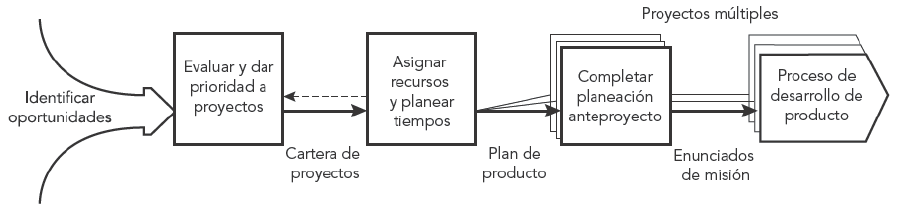
\includegraphics[width=.8\textwidth]{Figures/elproceso.png}
	\decoRule
	\caption{Proceso de planeaci\'on de un producto}
	\label{fig:elproceso}
\end{figure}

\subsection{Discapacidad en M\'exico}

De acuerdo con la Clasificaci\'on Internacional del Funcionamiento, de la Discapacidad y de la Salud, presentada en 2001, las personas con discapacidad “son aquellas que tienen una o más deficiencias f\'isicas, mentales, intelectuales o sensoriales y que al interactuar con distintos ambientes del entorno social pueden impedir su participaci\'on plena y efectiva en igualdad de condiciones a las dem\'as”.

Al año 2010, las personas en M\'exico que tienen alg\'un tipo de discapacidad son 5 millones 739 mil 270, lo que representa 5.1\% de la población total.\\
Una de las dificultades m\'as importantes a nivel nacional es la de caminar o moverse. Que referencia a la dificultad de una persona para moverse, caminar, desplazarse o subir escaleras debido a la falta de toda o una parte de sus piernas; incluye tambi\'en a quienes teniendo sus piernas no tienen movimiento o presentan restricciones para moverse, de tal forma que necesitan ayuda de otras persona, silla de ruedas u otro aparato, como andadera o pierna artificial.

\begin{figure}[th]
	\centering
	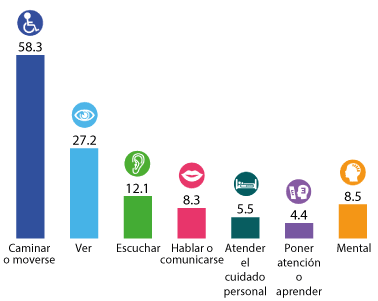
\includegraphics[width=.8\textwidth]{Figures/dificultad.png}
	\decoRule
	\caption{Porcentaje de la poblaci\'on con discapacidad seg\'un dificultad en la actividad (Año 2010)}
	\label{fig:elproceso}
\end{figure}

Algunos otros datos estad\'isticos sobre discapacidad en M\'exico que nos permitir\'an segmentar mejor el mercado para poder ofrecer un producto de valor para la poblaci\'on afectada por esta dificultad son:

\begin{itemize}
\item Las dificultades para caminar y para ver son las m\'as reportadas entre las personas con discapacidad.
\item Los principales detonantes de discapacidad en el pa\'is son las enfermedades (41.3\%) y la edad avanzada (33.1\%).
\item 23.1\% de la poblaci\'on con discapacidad de 15 años y m\'as no cuentan con alg\'un nivel de escolaridad.
\item De la poblaci\'on con discapacidad, 83.3\% es derechohabientes o est\'a afiliada a servicios de salud.
\item Participa en actividades económica 39.1\% de la poblaci\'on con discapacidad de 15 años y más, frente a 64.7\% de su contraparte sin discapacidad
\end{itemize}


\section{Modelo de negocio}

 
% Chapter 2

\chapter{Propuesta tecnol\'ogica} % Main chapter title

\label{Chapter3} % For referencing the chapter elsewhere, use \ref{Chapter1} 

%----------------------------------------------------------------------------------------

% Define some commands to keep the formatting separated from the content 

%----------------------------------------------------------------------------------------
Dada la introducci\'on correspondiente, en este cap\'itulo se describe la
propuesta tecnol\'ogica que compete a este proyecto, para esto se propone, en
particular, articular una soluci\'on que se identifique en el \'area de las
\emph{smart wheelchair} 
\section{Silla de ruedas inteligente}
Una silla de ruedas inteligente \emph{smart} es cualquier silla auto propulsada
que utiliza un sistema de contro para aumentar o incluso reemplazar el control
del usuario \parencite{smart}. Su prop\'osito es el de reducir o eliminar las
acciones del usuario para conducir la silla. Usualmente, una silla de ruedas
inteligente es controlada v\'ia una computadora, tiene una colecci\'on de
sensores y aplica t\'ecnicas de mobilidad de la rob\'otica, pero todo esto no es
exclusivamente necesario. La interfaz puede consistir de un joystick tradicional
de silla de ruedas, un dispositivo \emph{sip-and-puff} \footnote{tecnolog\'ia
que mediante inalaciones el usuario puede utilizar para indicar acciones}, o
alguna pantalla sensible al tacto. Estas en particular difieren de cualquier
otra silla de ruedas motorizada en el sentido en que, en estas \'ultimas el
usuario es quien controla la velocidad y direcci\'on del veh\'iculo por
completo, en una \emph{smart wheelchair} esta tarea es apoyada por el sistema de
control de la misma.\\
Las sillas de ruedas inteligentes son dise\~nadas para una gran variedad de
tipos de usuarios. Algunas son dise\~nadas para usuarios con deficiencias
cognitivas, como la demencia, estas comunmente son acondicionadas con sistemas y
t\'ecnicas de evaci\'on de colisiones logrando que incluso aunque el usuario lo
indique, estas no incurran en una situaci\'on de choque que pueda lastimar al
usuario. Algunas otras se enfocan en servir a pacientes con severas
discapacidades motoras, como la par\'alisis cerebral y/o la cuadraplejia y el
roll de la silla de ruedas es el de interpretar peque\~nas activaciones
musculares como comandos de alto nivel y ejecutarlos. Estas sillas por lo
general emplean t\'ecnicas de la inteligencia artificial, como la planeaci\'on
de trayectorias.

\section{Componentes}

\tikzstyle{block} = [draw, fill=blue!20, rectangle, 
    minimum height=3em, minimum width=6em]
\tikzstyle{sum} = [draw, fill=blue!20, circle, node distance=2cm]
\tikzstyle{input} = [coordinate]
\tikzstyle{output} = [coordinate]
\tikzstyle{pinstyle} = [pin edge={to-,thin,black}]

\begin{figure}
    \centering
% The block diagram code is probably more verbose than necessary
\begin{tikzpicture}[auto, node distance=3cm,>=latex']
    % We start by placing the blocks
    \node [input, name=input] {};
    \node [block, right of=input] (interfaz) {Intefaz};
    \node [sum, right of=interfaz] (sum) {};
    \node [block, right of=sum] (controlador) {Control};
    \node [block, right of=controlador] (power) {Potencia};
    \node [block, below of=controlador] (measurements) {Sensores};
    % We draw an edge between the controller and system block to 
    % calculate the coordinate u. We need it to place the measurement block. 
    \node [output, right of=power] (output) {};

    % Once the nodes are placed, connecting them is easy. 
    \draw [draw,->] (input) -- node {usuario} (interfaz);
    \draw [->] (interfaz) -- node {} (sum);
    \draw [->] (sum) -- node {} (controlador);
    \draw [->] (controlador) -- node {} (power);
    \draw [->] (power) -- node [name=y] {carga}(output);
    \draw [->] (y) |- (measurements);
    \draw [->] (measurements) -| node[pos=0.99] {$+$} 
        node [near end] {} (sum); 
\end{tikzpicture}
\caption{Definici\'on esquem\'atica de la soluci\'on}
\label{fig:esquemas}
\end{figure}


Como se muestra en la figura \ref{fig:esquemas} se proponen los siguientes
componentes para la composici\'on final de la soluci\'on:
\begin{itemize}
    \item Interfaz de usuario
    \item Sistema de control
    \item Sistema de potencia
    \item Sensores
\end{itemize}

\subsection{Esquema f\'isico}

\begin{figure}[th]
    \centering
    \includegraphics[width=.8\textwidth]{Figures/whelchair.jpg}
    \decoRule
    \caption{Silla de ruedas tradicional y manual}
    \label{fig:manual}
\end{figure}

Adem\'as de que, los componentes antes mencionados ser\'an descritos a
profundidad en las siguientes secciones, cabe aclarar que, como parte de la
propuesta de soluci\'on, se plantea el hecho de que dichos sistemas ser\'an
integrados sobre una silla de ruedas tradicional. ref.\ref{fig:manual}

Siendo as\'i podemos catalogar en este momento a esta propuesta como un
\emph{upgrade} m\'as que como un producto nuevo, a\'un as\'i como es descrito en
el cap\'itulo \ref{Chapter2} existe una necesidad real en el mercado por una
alternativa m\'as sofisticada en sectores de la sociedad no tan favorecidos.

\section{Interf\'az de usuario}

\begin{figure}[th]
    \centering
    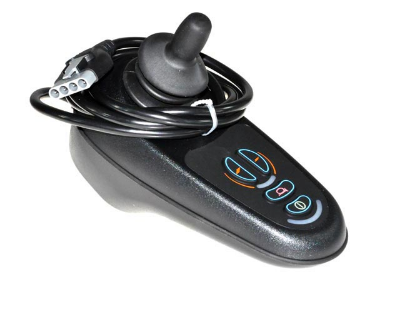
\includegraphics[width=.4\textwidth]{Figures/joystick.png}
    \decoRule
    \caption{Joystick tradicional}
    \label{fig:joystick}
\end{figure}
En este apartado se opta por ir con un sistema tradicional, dado que seg\'un las
observaciones del mercado que se hicieron en el ca\'pitulo \ref{Chapter2},
existe una gran demanda en el sector de los usuarios de sillas de ruedas con
capacidad motriz para operar un \emph{joystick} y aunado a la generosa oferta en
el mercado de dispositivos de este estilo, esto es determinado.\\



\section{Sistema de control}

Se propone un sistema de control autom\'atico para la \emph{silla smart} este
tendr\'a las siguientes tareas:
\begin{itemize}
    \item Procesar la se\~nal proveniente del joystick de control
    \item Interpretar las distintas se\~nales provenientes de los sensores
    \item Generar la salida adecuada para el sistema de potencia
\end{itemize}

Una de las consideraciones al momento de desarrollar dicho sistema de control es
que: \textbf{el usuario final ser\'a quien dirija la silla de ruedas} pero \textbf{el
sistema de control de la silla asistir\'a dicha conducci\'on.}\\

Con lo anterior planteado el sistema de control propuesto tendr\'a una tarea
bastante delimitada y se propone que resida en una computadora a bordo, el
detalle de su implementaci\'on se discute en el siguiente cap\'itulo.


\section{Sistema de potencia}

\subsection{Almacenamiento}

\begin{figure}[th]
    \centering
    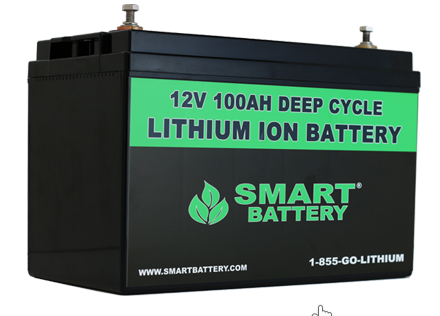
\includegraphics[width=.4\textwidth]{Figures/batery.png}
    \decoRule
    \caption{Banco de baterias; $12v$}
    \label{fig:batery}
\end{figure}

Para satisfacer a todo el sistema de energ\'ia se propone el uso de bater\'ias
el\'ectricas abordo. Dada la informaci\'on expuesta en el cap\'itulo
\ref{Chapter1} se elige el uso de las bater\'ias que entregar\'an una mejor
relaci\'on de densidad energ\'etica: las bater\'ias de iones de litio.\\
Dado que es un est\'andar en las sillas de ruedas motorizadas el uso de dos
bancos de baterias de $12v$ cada una, en este caso se opta por seguir con dicha
tendencia

\subsection{Entrega de potencia}

\begin{figure}[th]
    \centering
    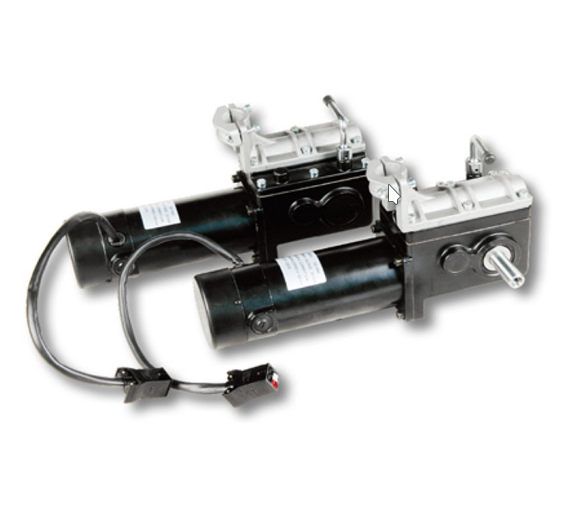
\includegraphics[width=.5\textwidth]{Figures/motor.png}
    \decoRule
    \caption{Par de motores de DC}
    \label{fig:motor}
\end{figure}

Para la entrega de potencia a la silla se utilizar\'an un par de motores de
corriente directa (fig.\ref{fig:motor}) acoplados sobre un chasis debajo del asiento de la silla
tradicional y directamente conectados a las ruedas estos contar\'an tambien con
un par de encoders \'opticos y el correspondiente controlador, mismos en los que
se aunar\'a en su descripci\'on en el siguiente cap\'itulo

\section{Sensores}

Con la intenci\'on de dotar al sistema de una retroalimentaci\'on que permita al
usuario final una experiencia de conducci\'on m\'as rica y sencilla, se pretende
incorporar en la soluci\'on distintos sensores, entre los que se encuentran,
pero no exclusivamente:
\begin{itemize}
    \item Sensores ultras\'onicos
    \item Sensores de nivel de bateria
    \item Aceler\'ometros
    \item Girosc\'opios
    \item Sensores de presi\'on
\end{itemize}

% Chapter 2

\chapter{Desarrollo e implementaci\'on} % Main chapter title

\label{Chapter4} % For referencing the chapter elsewhere, use \ref{Chapter1} 

%----------------------------------------------------------------------------------------

% Define some commands to keep the formatting separated from the content 

%----------------------------------------------------------------------------------------

\section{Dise\~no estructural}
\section{Hardware}
\section{Software}
\section{Sistema de seguridad}

 
% Chapter 2

\chapter{Conclusiones} % Main chapter title

\label{Chapter5} % For referencing the chapter elsewhere, use \ref{Chapter1} 

%----------------------------------------------------------------------------------------

% Define some commands to keep the formatting separated from the content 

%----------------------------------------------------------------------------------------

\section{Resultados obtenidos}
La investigaci\'on realizada para poder sentar las bases para el desarrollo de un producto como lo es la silla de ruedas motorizada nos deja reflexiones muy significativas. Por una parte el reconocimiento de la poblaci\'on discapacitada del pa\'is que hoy se encuentra con muchas dificultades para poder desenvolverse en la sociedad y que dadas las condiciones socioecon\'omicas, de desarrollo y de salud del pa\'is se ven potencializados los retos a los cuales esta poblaci\'on se tiene que enfrentar a fin de lograr calidad de vida y precisamente a este punto la relevancia de nuestra profesi\'on como desarrolladores de tecnolog\'ia al servicio de la patria.//
La segunda reflexi\'on es en el aspecto de nuestra formaci\'on, de la cual estamos completamente orgullosos y satisfechos pues como futuros egresados de la Facultad de Ingenier\'ia y de la carrera de Ingenier\'ia Mecatr\'onica hoy tenemos la capacidad de planificar, diseñar y desarrollar un producto integral que genere valor para la sociedad.//
Los resultados obtenidos en este trabajo nos motivan a creer que tenemos la capacidad para desarrollar tecnolog\'ia y soluciones ingenieriles cien por ciento mexicanas.
 

%----------------------------------------------------------------------------------------
%	THESIS CONTENT - APPENDICES
%----------------------------------------------------------------------------------------

\appendix % Cue to tell LaTeX that the following "chapters" are Appendices

% Include the appendices of the thesis as separate files from the Appendices folder
% Uncomment the lines as you write the Appendices

% Appendix A

\chapter{Frequently Asked Questions} % Main appendix title

\label{AppendixA} % For referencing this appendix elsewhere, use \ref{AppendixA}

\section{How do I change the colors of links?}

The color of links can be changed to your liking using:

{\small\verb!\hypersetup{urlcolor=red}!}, or

{\small\verb!\hypersetup{citecolor=green}!}, or

{\small\verb!\hypersetup{allcolor=blue}!}.

\noindent If you want to completely hide the links, you can use:

{\small\verb!\hypersetup{allcolors=.}!}, or even better: 

{\small\verb!\hypersetup{hidelinks}!}.

\noindent If you want to have obvious links in the PDF but not the printed text, use:

{\small\verb!\hypersetup{colorlinks=false}!}.

%\include{Appendices/AppendixB}
%\include{Appendices/AppendixC}

%----------------------------------------------------------------------------------------
%	BIBLIOGRAPHY
%----------------------------------------------------------------------------------------

\printbibliography[heading=bibintoc]

%----------------------------------------------------------------------------------------

\end{document}  
